\documentclass[a4paper,titlepage,11pt,oneside]{article}

\usepackage[utf8]{inputenc}
\usepackage[basque]{babel}
\usepackage[left=20mm, right=20mm, top=25mm, bottom=20mm]{geometry}
\usepackage{graphicx}
\usepackage{array}
\usepackage{fancybox}
\usepackage{multirow}

\usepackage[usenames,dvipsnames]{color}
\usepackage[
    bookmarks=true,
    unicode=true,
    pdftitle={Freedom for Hardware and Communications},
    pdfsubject={f4hc},
    pdfauthor={ITSAS},
    linktoc=all,
    colorlinks=true,
    linkcolor=Blue,
    urlcolor=BlueViolet,
    citecolor=Blue,
    ]{hyperref}

\definecolor{claro}{RGB}{99,200,25}
\definecolor{oscuro}{RGB}{0,135,0}
\definecolor{charla}{RGB}{0,169,157}
\definecolor{social}{RGB}{250,150,30}

\parskip=2mm

\usepackage{eso-pic}
\newcommand\BackgroundPic{
\put(0,0){
\parbox[b][\paperheight]{\paperwidth}{%
\vfill
\centering

\includegraphics[width=\paperwidth,height=\paperheight,
keepaspectratio]{f4hc_back.png}%
\vfill
}}}

\begin{document}

\pagestyle{empty}

\AddToShipoutPicture{\BackgroundPic}

\begin{center}
\begin{tabular}{ m{6.5cm} m{9cm} }
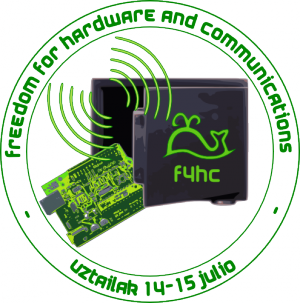
\includegraphics[width=150pt]{./logo_f4hc.png}
&
\begin{minipage}{9cm}
Antolatzailea:
\begin{center}

\includegraphics[width=100pt]{./itsas.png}
\end{center}

Babesleak:
\begin{center}

\includegraphics[width=100pt]{./upv_ehu.png}
\hspace{0.5cm}
\centering
\includegraphics[width=100pt]{./cenatic.png}
\end{center}
\end{minipage}
\\
\end{tabular}
\end{center}

\Large
\textbf{{\color{claro}Uztailak 14, ostegun goiza:} {\color{oscuro}Komunikazioak}}

\normalsize
{\color{social}\textbf{09:00}} Harrera

{\color{charla}\textbf{09:15}} Asterisk, erabilera anitzeko IP telefonogunea - Iker Sagasti

{\color{charla}\textbf{10:00}} SIP protokoloa IP-tik haratago - Saúl Ibarra

{\color{social}\textbf{10:45}} Atsedenaldia 

{\color{charla}\textbf{11:15}} HSMMN proiektua, irrati eta IP gaineko ahotsaren bateratzea - Alex Casanova

{\color{charla}\textbf{12:00}} ifreeTablet, software askea erabiltzen duen tablet askea - Jose Luis Aparicio

{\color{charla}\textbf{12:45}} Arduino proiektua - David Cuartielles

{\color{social}\textbf{13:45}} Saioaren amaiera

\Large
\textbf{{\color{claro}Uztailak 14, ostegun arratsaldea:} {\color{oscuro}Guifi}}

\normalsize
{\color{charla}\textbf{16:00}} Tempest eta beste informazio jario batzuk - Pablo Garaizar

{\color{charla}\textbf{16:45}} guifi.net errEboluzioa

{\color{social}\textbf{17:30}} Atsedenaldia 

{\color{charla}\textbf{18:00}}Haririk gabeko teknologiadun Mesh sareak: alderdi tekniko eta sozialak - Pau Escrich

{\color{charla}\textbf{19:00}} Guifi EH, Catalunyako sare askea Euskal Herrira heldu da - Joseba Senosiain

{\color{social}\textbf{19:30}} Saioaren amaiera

{\color{social}\textbf{21:30}} Emaileekin afaria

\Large
\textbf{{\color{claro}Uztailak 15, ostiral goiza:} {\color{oscuro}Hardware askea}}

\normalsize
{\color{charla}\textbf{09:30}} Kontsumo txikiko ordenagailuak: SheevaPlug - Jorge Cacho

{\color{charla}\textbf{10:00}} Artearen egoera estandar irekien bidezko mugikorrentzako plataforma anitzeko aplikazioen garapenean - Iker Pérez de Albéniz

{\color{social}\textbf{10:45}} Atsedenaldia 

{\color{charla}\textbf{11:15}} OpenLase, laser bidezko realtime proiekzioa - Hector Martín

{\color{charla}\textbf{12:15}} Hardware copyleft, Qi-hardware komunitatea - David Reyes

{\color{social}\textbf{13:30}} Jardunaldien amaiera 

\begin{center}
\Huge{\textbf{\color{oscuro}http://itsas.ehu.es/f4hc}}
\end{center}
\end{document}